\textbf{Пример 1}

Рассмотрим следующий вызов функции:

\t{construct([[1, 1, 2, 2], [1, 1, 2, 2], [2, 2, 1, 2], [2, 2, 2, 1]])}

В этом примере требуется, чтобы существовал ровно 1 путь от башни $0$ до башни $1$. Для каждой из остальных пар башен $(x, y)$ таких, что $0 \leq x < y \leq 3$, должно существовать ровно два пути от башни $x$ до башни $y$.

Требуемой конфигурции можно достичь с помощью $4$ мостов, соединяющих пары башен $(0, 1)$, $(1, 2)$, $(1, 3)$ и $(2, 3)$.

Для того, чтобы сообщить описанную выше конфигурацию мостов, функция \t{construct} должна совершить следующий вызов функции:
\begin{itemize}
\item \t{build([[0, 1, 0, 0], [1, 0, 1, 1], [0, 1, 0, 1], [0, 1, 1, 0]])}
\end{itemize}

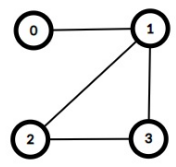
\includegraphics{Supertrees.png}

После этого функция \t{construct} должна вернуть $1$.

В данном примере существует несколько возможных ответов, удовлятворяющих всем требованиям архитектора, любой из которых будет считаться верным.

\textbf{Пример 2}

Рассмотрим следующий вызов функции:

\t{construct([[1, 0], [0, 1]])}

В этом примере требуется, чтобы ни от одной башни до другой не существовало пути. Требуемой конфигурции можно достичь только полным отсутствием мостов.

Для этого функция \t{construct} должна совершить следующий вызов функции:
\begin{itemize}
\item \t{build([[0, 0], [0, 0]])}
\end{itemize}

После этого функция \t{construct} должна вернуть $1$.

\textbf{Пример 3}

Рассмотрим следующий вызов функции:

\t{construct([[1, 3], [3, 1]])}

В этом примере требуется, чтобы существовало $3$ различных пути от башни $0$ до башни $1$. Не существует конфигурации мостов, которая удовлетворяла бы этим требованиям.
В этом случае функция \t{construct} должна вернуть $0$ без каких-либо вызовов функции \t{build}.
